\section{INTRODUCTION}
\label{sec:introduction}

In the distant past, meteorites of enormous size flew through the Earth's atmosphere and crashed into our planet; these collisions vaporized mineral fragments from the ground and sent them into the sky. The molten minerals floated in the air like sparkling raindrops, each one traveling thousands of kilometers before falling back to the ground. Even further back, the collision of two hot celestial bodies caused the formation of the Earth and the Moon as we know them today, with the Earth carrying a multitude of minerals within it. After millions of years buried under layers of rock, these shiny mineral fragments occasionally rose to the surface to tell of the vastness of the Earth and the immensity of time.

Geology is the study and combination of knowledge about how rocks form over thousands of years, how fascinating gemstones can be created under pressure and temperature, how minerals are formed, and also about fossils and geological heritage. The Earth was formed about 4.6 billion years ago, so there must be beautiful formations of rare rocks, or even gemstones hidden somewhere within the Earth. Therefore, learning about the theory of rocks and minerals through books will only get us halfway through the actual knowledge of Earth geology. As President Ho Chi Minh taught us: "Learning must go hand in hand with practice. It is useless to study without practice; if you don't learn, you won't be fluent."

Therefore, we went on a trip to visit the Ho Chi Minh City Geological Museum as part of a learning activity, to practice observing and understanding the geological history of Vietnam, with the formation of rocks, ores, minerals, and even gemstones.

\subsection{Museum Overview and Visit Objectives}
\label{subsec:museum-overview}

\begin{figure}[H]
  \centering
  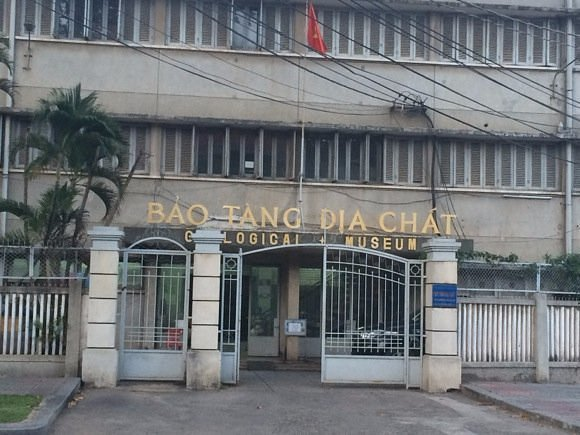
\includegraphics[width=0.8\textwidth]{graphics/figure_01.jpg}
  \caption{Ho Chi Minh City Geological Museum}
  \label{fig:museum}
\end{figure}

The visit to the Ho Chi Minh City Geological Museum provided us with a valuable chance to connect the theories we learned in class with real-world examples. While books and lectures give us the foundation of geological knowledge, nothing compares to directly observing the specimens that reflect millions, even billions, of years of Earth's history. At the museum, we could see how rocks, ores, minerals, and gemstones are preserved and displayed, each telling a story about the planet's formation and transformation over time.

This experience not only strengthened our understanding of the processes that shape the Earth but also gave us a clearer view of Vietnam's own geological heritage. By exploring these collections, we were able to develop a deeper appreciation of geology as both a science and a record of natural history. More importantly, the museum visit allowed us to practice critical observation, linking theory with practice, and to better prepare for future studies and projects related to Earth sciences.

\subsection{Museum History and Significance}
\label{subsec:museum-history}

The Geological Museum has a long history closely tied to the development of geological research in Vietnam since the colonial period. In 1898, the French colonial government established the Indochina Geological Service (Service Géologique de l'Indochine) and initiated the construction of a museum dedicated to geological research and education. By 1914, the museum's first building was completed in Hanoi. After the Geneva Agreement in 1954, part of the collection was moved to Saigon, where it was initially displayed in a temporary villa before being relocated to its current building in 1973. Following national reunification, the museum was managed by the Southern Geological Mapping Federation and continued to expand within the national geological system.

In 2001, it became one of the first museums in Vietnam to be recognized by the International Council of Museums (ICOM). In 2003, the Geological Museum system was restructured under the Department of Geology and Minerals, and in 2008, the Ho Chi Minh City branch was officially integrated as the southern division. Today, the Geological Museum stands as Vietnam's national geological museum, operating under the Department of Geology and Minerals of the Ministry of Natural Resources and Environment.

The museum currently holds about 13,000 precious geological specimens, of which about 3,000 are on permanent display. Including geological drill cores and archived samples, the total number of specimens here is more than 20,000. The highlight on the ground floor (General Geology) is the 1:500,000 scale geological map of Vietnam completed in 1988. This large map shows the geological structure of the entire territory of Vietnam clearly annotated, very useful for visitors to learn about the diversity of resources and stratigraphy.

This report will illustrate our visit to the Ho Chi Minh City Geological Museum, particularly focusing on Floor 1 and Floor 2. The first floor of the Museum will briefly introduce the geological evolution of Vietnam with the geological processes. On the second floor, we will demonstrate the fuel, metallic and non-metallic minerals, gemstones, mineral water and the concept of geological heritage. Throughout this report, we will organize the geological knowledge and our own experience to make this report more informative and easier to comprehend.